\documentclass[10pt,a4paper]{extarticle}
\usepackage[latin1]{inputenc}
\usepackage{amsmath}
\usepackage{microtype}
\usepackage[none]{hyphenat}
\usepackage{verbatim}
\usepackage{amsfonts}
\usepackage{amssymb}
\usepackage{enumitem}
\renewcommand{\familydefault}{\sfdefault}
\usepackage{mathpazo}
\renewcommand{\rmdefault}{put}
\usepackage{enumitem}
\usepackage[dvipsnames,svgnames]{xcolor}
\usepackage{tkz-euclide}
\usetkzobj{all}
\usepackage{graphicx}
\usepackage{subcaption}
\usepackage{tikz} 	
\usepackage{adjustbox}
\usepackage{multicol}
\usepackage{lipsum}
\usepackage[left=0.7cm,right=1cm,top=1cm,bottom=1.5cm]{geometry}
\usepackage{cancel} \usepackage{xcolor}
\usepackage{tcolorbox}
\usetikzlibrary{decorations.pathmorphing,patterns}
\usetikzlibrary{decorations.pathreplacing,calc}
 \newcommand\coret[2][red]{\renewcommand\CancelColor{\color{#1}}\cancel{#2}}
\SetLabelAlign{Center}{\hfil\makebox[1.0em]{#1}\hfil}

%%_------= solusi


% Set this =0 to hide, =1 to show

% Set this =0 to hide, =1 to show
\newtcolorbox{mybox}[1][] { colframe = blue!10, colback = blue!3,boxsep=0pt,left=0.2em, coltitle = blue!20!black, title = \textbf{jawab}, #1, } 

%---------- kunci (jika 1 ) muncul
\def\tampilkunci{1}
\newcommand{\hide}[1]{\ifnum\tampilkunci=1
%
\begin{mybox}
 #1
\end{mybox}
%
\vspace{\baselineskip}\fi}



\newcommand*\cicled[1]{\tikz[baseline=(char.base)]{\node[white, shape=circle, fill=red!80,draw,inner sep=0.5pt](char){#1};}}

\newcommand*\kunci[1]{\ifnum\tampilkunci=1
%
\tikz[baseline=(char.base)]{\node[red, shape=circle,draw,inner sep=0.5pt,xshift=2pt](char){#1};}\stepcounter{enumii}
\fi\ifnum\tampilkunci=0
%
\hspace{3pt}#1\stepcounter{enumii}
%
\fi}

\newcommand*\silang[1]{\tikz[baseline=(char.base)]{
\draw[red,thick](-0.2,-0.20)--(0.2,0.2);
\draw[red,thick](-0.2,0.20)--(0.2,-0.2);
\node[black](char){#1};
}}

\newcommand*\centang[1]{\tikz[baseline=(char.base)]{
\draw[red, very thick](-0.2,0.1)--(-0.1,0)--(0.2,0.3);
\node(char){#1};
}}

\newcommand*\merah[1]{
\textcolor{red}{#1}}
\newcommand*\pilgan[1]{
\begin{enumerate}[label=\Alph*., itemsep=0pt,topsep=0pt,leftmargin=*,align=Center] #1 
\end{enumerate}}
\newcommand*\pernyataan[1]{
\begin{enumerate}[label=(\arabic*), itemsep=0pt,topsep=0pt,leftmargin=*] #1 
\end{enumerate}}

\newcommand{\pilgani}[1]{                            \vspace{-0.3cm}\begin{multicols}{2}
 \begin{enumerate}[label=\Alph*., itemsep=0pt,topsep=0pt,leftmargin=*,align=Center]#1                     \end{enumerate}
 \phantom{ini cuma sapi, wedus, dan ayam}
 \end{multicols}}


\begin{document}


 \textbf{Gerak Harmonik Sederhan} \phantom{ini nama siswa yang aaamengerjakan soal kuis ini }  

\begin{multicols*}{2}\raggedcolumns
\textbf{Persamaan Gerak Harmonik}\\
Gerak harmonik adalah gerak bolak-balik suatu titik keseimbangan secara teratur. Bayangkan bagaimana gerak suatu bandul, atau gerakan pegas yang digantungi massa, ditarik kemudian dilepaskan.\\
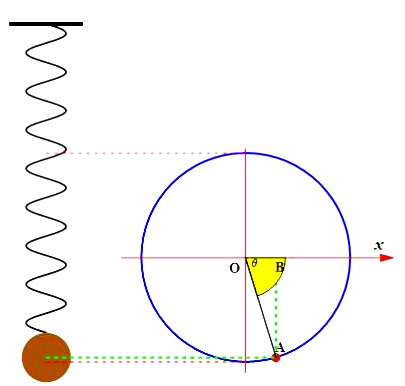
\includegraphics[height=6.5cm]{pic/kuis-ghs1}

Pada gerak harmonik, gerakan naik turun pegas bisa dianggap sebagai gerak melingkar yang dilihat dari samping. Saat menyimpang maksimal terjadi $A$ amplitudo. Simpangan $y$ pada setiap saat tergantung sudut yang dibentuk
\begin{align*}
y&=A\sin(\theta)\\
y&=A\sin(2\pi.\phi)\\
y&=A\sin(2\pi.f.t)\\
y&=A\sin(\omega.t)
\end{align*}
\setlength{\tabcolsep}{0.1\tabcolsep}

\begin{tabular}{p{0.5cm} p{1mm} p{6cm}}
$y$ &:& simpangan \\
$v$ &:& kecepatan \\
$a$ &:& percepatan \\
$A$ &:& amplitudo/simpangan maks (m)\\
$\theta$&:& sudut fase\\
$\phi$&:& fase getaran
\end{tabular}\\
\begin{align*}
\text{fase} &= \phi = \frac{t}{T}=f.t=\frac{\theta}{360}
\end{align*}
Perhatikan bagaimana menghitung sinus dan cosinus
\begin{align*}
\sin(50\pi) &= \sin(25x2\pi)\\
\text{padahal 1 putaran adalah }&2\pi\text{,sehingga kembali ke titik 0 lagi}\\
\sin(50\pi) &= \sin (0) = 0\\
\sin(7,5\pi) &= \sin (6\pi + 1,5\pi)\\
\sin(7,5\pi) &= \sin (1,5\pi) = \sin (270) = -1
\end{align*}

\textbf{Persamaan Kecepatan}
\begin{align*}
v&=A\omega \cos(\omega.t)\\
v&=A\omega\cos(\theta)
\end{align*}

\textbf{Persamaan Percepatan}
\begin{align*}
a &= -A\omega^2\sin(\omega.t)\\
a &= -A\omega^2\sin(\theta)
\end{align*}

\vspace{2cm}

\begin{enumerate}
\item Sebuah benda bergerak secara harmonis dengan persamaan $$y = 0,02 \sin (20\pi t) $$
Tentukan:
\begin{enumerate}[noitemsep,label=\alph*.]
\item Amplitudo
\item frekuensi
\item simpangan saat t = 1/40 s
\item simpangan saat sudut fasenya 60$^o$
\item persamaan kecepatannya
\item kecepatan maksimum
\item kecepatan saat t = 1/60 s
\item persamaan percepatannya
\item percepatan maksimum
\end{enumerate}
\vspace{6cm}

\item Sebuah benda melakukan gerak harmonik dengan frekuensi 10 Hz dan amplitudo 5 cm. Pada suatu saat simpangannya berada pada 3 cm. Berapa kecepatan benda saat itu?
\pilgani{
\item 50 cm/s
\item 50$\pi$cm/s
\item 100$\pi$ cm/s
\item 80$\pi$ cm/s
\item 80$\sqrt{3}\pi$ cm/s
}
\vspace{3cm}

\item Kecepatan suatu benda adalah setengah dari kecepatan maksimumnya. Jika simpangan maksimum benda adalah 6 cm, maka simpangannya saat itu adalah . . . .
\pilgani{
\item 3 cm
\item 3$\sqrt{3}$ cm
\item 6 cm
\item 3$\sqrt{2}$ cm
\item 0 cm
}
\vspace{5cm}

\textbf{Persamaan Osilasi Pegas dan Bandul  $\omega$}\\
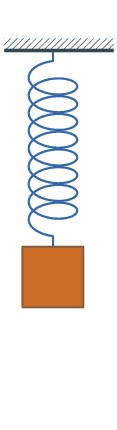
\includegraphics[height=4cm]{pic/pegas}
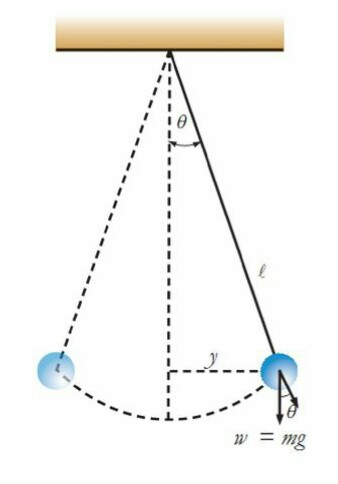
\includegraphics[height=4cm]{pic/bandul}

\begin{tabular}{p{2cm} p{2cm}}
$$\omega=\sqrt{\frac{k}{m}}$$ & $$\omega=\sqrt{\frac{g}{l}}$$ 
\end{tabular}
\vspace{3cm}

\item Sebuah pegas dengan konstanta 300 N/m digantungi oleh massa 3 kg. Maka frekuensi dan periode pegas tersebut adalah . . . .

\vspace{3cm}

\item  Bandul dengan panjang tali 40 cm digantungi beban, maka frekuensi dan periode bandul adalah . . . 
\vspace{3cm}


\item Bandul dengan panjang tali 10 cm digantungi beban dengan massa 200 gram. Jika amplitudo benda tersebut adalah 4cm, maka kecepatannya saat simpangannya 2cm adalah . . . .

\vspace{7cm}


\textbf{Persamaan Energi pada Getaran}




Getaran melakukan simpangan secara harmonik. Saat simpangan maksimal, benda bergetar akan berhenti lalu bali arah. Kecepatan maksimal justru akan diperoleh saat melewati titik keseimbangan.

\begin{align*}
E_{\text{total}}&=E_{\text{potensial}}+ E_{\text{kinetik}}\\
\frac{1}{2}k.A^2 &= \frac{1}{2}k.y^2+\frac{1}{2}k(A^2-y^2)
\end{align*}


\item Sebuah benda bermassa 3 kg bergetar dengan frekuensi $\frac{50}{\pi}$ Hz. Energi potensial saat simpangannya 2 cm adalah . . .  

\vspace{3cm}

\item Suatu benda begetar dengan simpangan maksimal 20 cm. Suatu saat benda memiliki energi potensial tiga kali energi kinetik. Tentukan berada simpangan saat itu! . . . 
\vspace{4cm}

\item Benda bergetar dengan frekuensi 10Hz. Benda tersebut pada suatu saat energi kinetiknya 4 kali energi potensial. Jika amplitudo adalah 4 cm, maka simpangan saat itu adalah . . . 
\vspace{4cm}

\item Sebuah benda yang massanya 100 gram bergetar harmonik dengan periode $\frac{1}{5}$ detik dan amplitudo 2 cm. Besar energi kinetiknya pada saat simpangan 1 cm adalah . . .
\pilgani{
   \item $7,50 \pi^2 \times 10^{-3}$ joule
   \item $5,00 \pi^2 \times 10^{-3}$ joule
   \item $3,75 \pi^2 \times 10^{-3}$ joule
   \item $2,50\pi^2 \times 10^{-3}$ joule
   \item $1,50 \pi^2 \times 10^{-3}$ joule
}
\vspace{3cm}
\item Suatu ayunan bandul sederhana menggunakan tali yang panjangnya 40m memiliki periode 1 s. Jika nilai $\pi^2=10$ maka percepatan gravitsi di tempat itu adalah . . .
\pilgani{
   \item 10 m/s$^2$
   \item 9,4 m/s$^2$
   \item 9,8 m/s$^2$
   \item 9,2 m/s$^2$
   \item 9,6 m/s$^2$}
\vspace{3cm}

\item Dua pegas masing-masing konstantanya 100 N/m. Ujung bawah pegas digantungi beban 4 kg. Perbandingan energi potensialnya, jika pegas disusun paralel dan disusun seri adalah . . .
\pilgani{
   \item 1 : 4
   \item 1 :  2
   \item 1 : 1
   \item 2 : 1
   \item 4 : 1
}
\vspace{3cm}

\item Sebuah partikel melakukan ayunan harmonis sederhana. Tenaga kinetik partikel adalah $E_k$ dan tenaga potensialnya $E_p$, tenaga totalnya adalah $E_T$. Ketika partikel berada di tengah-tengah antara posisi simbang dan posisi amplitudo, perbandingan $E_K/E_T$ dan $E_p/E_T$ berturut-turut adalah . . .
\pilgani{
   \item 1/4 dan 3/4
   \item 1/2 dan 1/2
   \item 3/4 dan 1/4
   \item 1/8 dan 7/8
   \item 3/8 dan 5/8
}
\vspace{3cm}

\item Sebuah partikel bermassa 10 gram bergetar harmonis dengan frekuensi 100Hz dan amplitudo 8 cm. Energi potensialnya pada saat sudut fasenya 300$^o$ adalah . . . 
\pilgani{
   \item 0,12$\pi^2$
   \item 0,24$\pi^2$
   \item 0,36$\pi^2$
   \item 0,48$\pi^2$
   \item 0,96$\pi^2$}
\vspace{3cm}

\item Jika simpangan sebuah benda yang bergetar harmonik sama dengan setengah amplitudonya, pada saat itu fasenya adalah  . . . .  (fase $\phi=\frac{\theta}{360}$)
\pilgani{
   \item $\frac{1}{2}$
   \item $\frac{1}{4}$
   \item $\frac{1}{6}$
   \item $\frac{1}{8}$
   \item $\frac{1}{12}$}
   \vspace{3cm}

   \item Sebuah partikel bergetar harmonik dengan amplitudo 20 cm. Jika suatu saat energi kinetik partikel sama dengan energi potensialnya, besar simpangannya adalah . . .
   \pilgani{
      \item 20 cm
      \item 20$\sqrt{2}$ cm
      \item 10 cm
      \item 10$\sqrt{2}$ cm
      \item 5$\sqrt{2}$ cm
   }
   \vspace{2cm}

   \item Sebuah bandul dengan massa 30 gram menyimpang sejauh 4 cm. Jika panjang tali adalah 1 m, maka gaya pemulihnya adalah . . . (* gaya pemulih $F=mg \sin (\theta)$)\\ 
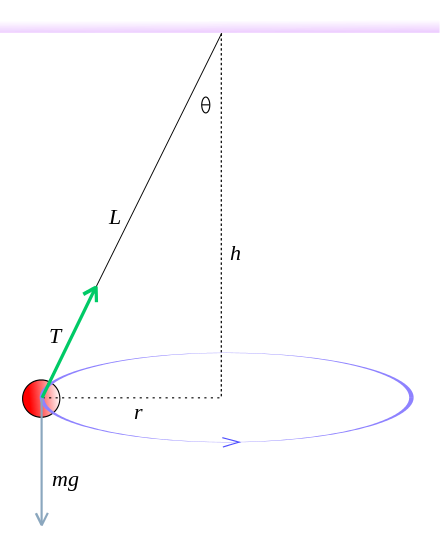
\includegraphics[width=4cm]{pic/pendulum} 
\pilgani{ \item 0,006 N
   \item 0,012 N
   \item 0,024 N
   \item 0,036 N
   \item 0,040 N
   }
   \vspace{2cm}

\item Percepatan partikel setelah bergetar 0,5 s pada persamaan simpangan $y = 4 \sin (\frac{\pi}{2}t)$ cm  adalah . . .
\pilgani{
   \item nol
   \item $-5\sqrt{2}$ cm/s$^2$
   \item $5\sqrt{2}$ cm/s$^2$
   \item $-5\sqrt{2}\pi^2$ cm/s$^2$
   \item $5\sqrt{2}\pi^2$ cm/s$^2$
}
\end{enumerate}
\end{multicols*}
\end{document}
